\documentclass{lug}
\usepackage{url}


\title{scikit-learn}
\author{C. Travis Johnson}
\date{April 27, 2017}
\institute{Mines Linux Users Group}

\begin{document}

\section{Introduction}
\subsection{Machine Learning}
\begin{frame}{Machine Learning - What is it really?}
    \begin{itemize}[<+->]
        \item Goal: Extract Knowledge from Data
        \item Sometimes called predictive analysis or statistical learning
        \item Given a large matrix of observations $X$, fit a function $f(x)$ that maps observation $x$ to a response variable $y$
    \end{itemize}
\end{frame}

\begin{frame}{Important Terms}
  \begin{description}
    \item[Classifiers] Algorithms that learn functions to map observations to a \textit{discrete} response. E.g., is this tumor malignant or benign? Is this
      email spam or not?
    \item[Regressors] Algorithms that learn functions to map observations to a \textit{continuous} response. E.g., how much should this house cost?
    \item[Underfitting] The learned function is too simple. ``We barely studied for the exam.''
    \item[Overfitting] The learned function is too complex. ``We memorized all the practice problems, but don't understand the material.''
    \item[Generalization] How well does the learned function extend to new observations?
  \end{description}
\end{frame}

\subsection{Scikit-Learn}
\begin{frame}{Scikit-Learn: Machine Learning in Python}
  \begin{itemize}[<+->]
    \item Provides many machine learning tools with a common \texttt{Estimator} interface\footnote{
        \url{http://scikit-learn.org/stable/developers/contributing.html\#apis-of-scikit-learn-objects}}
    \item Built in helpers for common ML tasks (e.g., \texttt{metrics}, \texttt{preprocessing})
    \item Easily combine algorithms to make a complex pipeline\footnote{Sound familiar?}
    \item Relies heavily on \texttt{numpy} and \texttt{scipy}, often used with \texttt{pandas}
  \end{itemize}
\end{frame}

\section{Supervised Learning}
\subsection{Example: Predicting Breast Cancer with Decision Trees}
\begin{frame}{Learning to Predict Breast Cancer}
\inputminted{python3}{examples/cancer-dt.py}
\end{frame}

\begin{frame}{Evaluating Accuracy of a Model}
\inputminted{python3}{examples/cancer-dt2.py}
\end{frame}

\begin{frame}{Other Supervised Learning Models}
  \begin{itemize}[<+->]
    \item Decision trees are a common first step, because they're easy to interpret and don't require much \texttt{preprocessing}
    \item Decision trees are prone to overfitting, so a good improvement is the \texttt{RandomForest}
    \item Support Vector Machines, Logistic/Linear Regression, and Artificial Neural Networks are commonly the first algorithms studied
    \item See the \texttt{scikit-learn} documentation for a comprehensive guide of available algorithms
  \end{itemize}
\end{frame}

\begin{frame}{Becoming a ``Data Scientist''}
  \begin{enumerate}
    \item Get some (more) data
    \item Pick an algorithm (or algorithm chain)
    \item Train the model
    \item Test generalization ability of trained model
    \item Good enough? Done. Else, go back to step 1 or 2.
  \end{enumerate}
  \begin{center}
  Then, tell people you're a genius \dots it's that easy!
  \end{center}
\end{frame}

\section{Unsupervised Learning}
\begin{frame}{Distinction from Supervised Learning}
  \begin{description}
    \item[Supervised Learning] You tell the model what the correct answers are for training examples.
    \item[Unsupervised Learning] You ask the model to extract information from a dataset.
    \item[Unsupervised Clustering] Partition data into similar groups. Example: K-Means Clustering
    \item[Unsupervised Transformations] Create new representations of data. Example: Principal Component Analysis
  \end{description}
\end{frame}

\section{Model Evaluation and Improvement}
\begin{frame}{Choice of Evaluation Metric}
  \begin{itemize}[<+->]
    \item Accuracy is not always the best metric for your system
    \item Plenty of others exist, pick the best for your business costs
    \item Look in the \texttt{sklearn.metrics} module for alternatives
    \item You can also use your own evaluation function!
  \end{itemize}
\end{frame}

\begin{frame}{Cross Validation}
  \begin{block}{Never Fit Models to Test Data! Ever!}
  Learning the parameters of a prediction function and testing it on the same data is a methodological mistake: a model that would just repeat the
  labels of the samples that it has just seen would have a perfect score but would fail to predict anything useful on yet-unseen data. This situation
  is called overfitting.
  \end{block}

  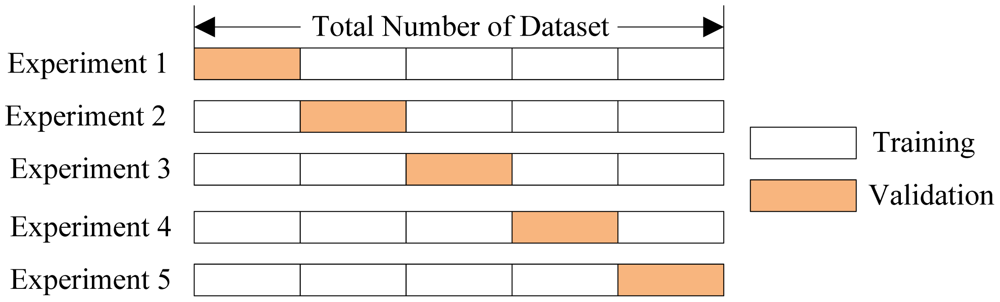
\includegraphics[width=\linewidth]{graphics/cv-explained}
\end{frame}

\begin{frame}{Grid Search with Cross Validation}
\inputminted[fontsize=\scriptsize]{python3}{examples/gridsearch.py}
\end{frame}

\section{Pipelines}
\begin{frame}{Pipelines}
  Use \texttt{Pipeline} to combine multiple estimators into a single estimator. Two conveniences:
  \begin{enumerate}
    \item Convenience: You only have to call fit and predict once on your data to fit a whole sequence of estimators.
    \item Joint parameter selection: You can grid search over parameters of all estimators in the pipeline at once.
  \end{enumerate}
\end{frame}

\begin{frame}{A Simple Pipeline}
  \inputminted[fontsize=\scriptsize]{python3}{examples/pipeline.py}
\end{frame}

\begin{frame}{Grid Search - Tuning a Complex Pipeline}
  \inputminted[fontsize=\scriptsize]{python3}{examples/gridsearch_pipeline.py}
\end{frame}

\begin{frame}[standout]
    \Huge
    Questions?
\end{frame}
\end{document}
